\documentclass[12pt]{standalone}

\usepackage{tikz}
\usetikzlibrary{decorations.markings}
\usetikzlibrary{math}

\newcommand\getLength[4]{sqrt((#1-#3)*(#1-#3) + (#2-#4)*(#2-#4))}


\begin{document}
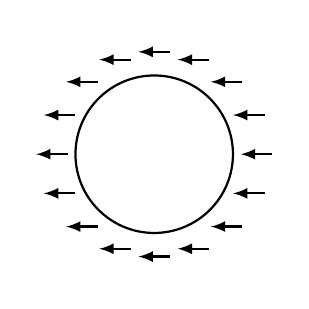
\begin{tikzpicture}

\draw[white] (-1.6,1.6) rectangle (1.6,-1.6);

% Number of arrows
\tikzmath{
    \n = 16;
    \step = 360/\n;
    \radius = 1.3;
    \radiuss = 0.4;
    \rotationalSpeed = 0.0;
}

\foreach \x in {1,...,\n} {

    % Sets up the line elements with correct rotations    
    \tikzmath{
        \xone = \radius*cos(\x*\step);
        \xtwo = \radius*sin(\x*\step);
        \yone = \radius*cos(\x*\step) + \radiuss*cos(\x*\rotationalSpeed*\step);
        \ytwo = \radius*sin(\x*\step) + \radiuss*sin(\x*\step*\rotationalSpeed);
        \R = \getLength{\xone}{\xtwo}{\yone}{\ytwo};
    }

    % Draws the vector
    \draw[thick,-latex] 
    ({\yone - 0.5*(\yone-\xone)},
    {\ytwo - 0.5*(\ytwo-\xtwo)})
    --
    ({\xone - 0.5*(\yone-\xone)},
    {\xtwo - 0.5*(\ytwo-\xtwo)});
}


% Draws the dashed line
\draw[
    thick,
    decoration={markings},
    postaction={decorate}
    ] 
    (0,0) circle (1cm);

\end{tikzpicture}
\end{document}